\documentclass{article}

\usepackage{times}
\usepackage{uist}
%\usepackage[config, font=small, labelfont={sf,bf}, textfont=sf]{caption,subfig}
\usepackage{caption,subfig}
\usepackage{graphicx}

\begin{document}

% --- Copyright notice ---
\conferenceinfo{UIST'11}{October 16-19, 2011, Santa Barbara, CA, USA}
\CopyrightYear{2011}
\crdata{978-1-4503-0716-1/11/10}

% Uncomment the following line to hide the copyright notice
\toappear{}
% ------------------------

\bibliographystyle{plain}

\title{Sketch It, Make It: Freehand Drawing for Precision Rapid Fabrication}

\author{
\parbox[t]{9cm}{\centering
	     {\em Author One}\\
	     Institution Name\\
             City, ST, USA\\
	     user@institution.net}
\parbox[t]{9cm}{\centering
	     {\em Author Two}\\
	     Institution Name\\
             City, ST, USA\\
	     user@institution.net}
}

\maketitle

% TODO: change this
\abstract Abstract goes here. 

\classification{I.3.5 [Computational Geometry and Object Modeling]: Modeling packages}

% TODO: change this
\terms{Design, Human Factors}

\keywords{sketching, rapid fabrication, design tools, constraints}

\tolerance=400 % prevent words from sticking out in the margin

%% \begin{figure}[tb]
%% \vspace{1.9in}
%% \caption{A figure caption.  It is set in 9 point Helvetica type, with a
%% 0.5 cm wider margin on both left and right sides.} 
%% \label{fig-example}
%% \end{figure}

\section{INTRODUCTION}

A growing community of self-described \textit{makers} design and build
many kinds of physical things~\cite{gershenfeld-fab}. Some are
electronic or robotic gizmos, while others are made from traditional
material. These ``new makers''~\cite{gross-new-makers} are empowered
by rapid fabrication machines like 3D printers and laser cutters.

It is possible that we are beginning to see a shift from an economy
based on mass-production (in factories) to one that includes
mass-customization (in homes, schools, and community
centers)~\cite{economist-fab}. Rapid fabrication machines continue to
decline in price while improving in quality. A new sector of
businesses use rapid fabrication to cater to the needs of hobbyist
designers as well as people that need highly customized
goods~\cite{nyt-rapidfab}.  For example, companies such as Ponoko
fabricate and send users physical output based on digital models
uploaded over the web.

Laser cutters are among the more popular rapid fabrication
machines. They can be thought of as a very fast, strong, and precise
automated razor blade, cutting through flat material (paper, wood,
plastic, metal, etc.) from directly above. Many items can be made
entirely with a laser cutter, aside from the occasional screw or glue.
Figure~\ref{fig:laser-example} shows several examples of useful items
made with laser cutters.

\begin{figure}[h]
\centering 
\subfloat[] {
  \label{fig:laser-example-a} 
  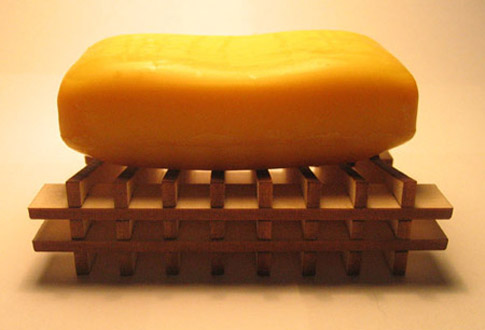
\includegraphics[width=0.4\linewidth]{img/flat-b.jpg}
}
\subfloat[] {
    \label{fig:laser-example-b}
    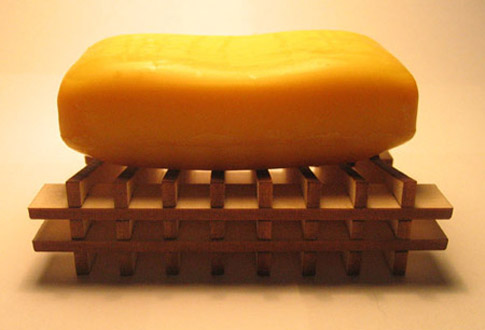
\includegraphics[width=0.4\linewidth]{img/flat-b.jpg}
}
\caption{Laser cut items.}
\label{fig:laser-example}
\end{figure}

Today, designers can choose among several modeling tools for laser
cutter projects. Adobe Illustrator, a general-purpose vector graphics
editor, is the most commonly used tool. Illustrator is full-featured
and has an interface new users find familiar. However, participants in
a formative study had a hard time using Illustrator quickly and
effectively when designing for laser cutters. Specialized CAD tools
like Rhino or SolidWorks are perhaps more appropriate for this kind of
modeling but they also have a substantial learning curve. If rapid
fabrication is to become common, appropriate modeling tools must be
made accessible to ordinary users~\cite{lipson-homefactory}.

Laser cut items are composed of parts cut from solid, flat pieces of
material. The primary concern of the designer is to define the path
taken by the laser cutter. Parts may be put together in various ways.
Pieces can be glued or screwed together in layers. Alternately the
user can design joints so the parts fit together. Most joints have
small margins of error. It is important that lengths, angles, and
relative position be indicated with precision for the parts to fit
together as they should.

In this paper, we present a modeling tool called ``Sketch It, Make
It'' (SIMI).  It is based on recognizing short sequences of sketched
input with a stylus. By using freehand drawn input, SIMI enables the
designer to iteratively and incrementally create laser cut models that
fit precise specifications.

We are inspired by the potential of freehand drawing as a basis for
our tool for several reasons. Sketching is quick and can be easily
learned. The technology is simple.  Unlike structured editing
software, a designer does not need to set the pencil's mode to line,
circle, or anything else. A freehand sketch can provide enough
information that others can translate it into a digital model. 

The primary contribution of this work is a system that embodies a new
way of designing precise 2D shapes by incremental sketch recognition
and rectification.

\subsection{Paper Organization}



\section{RELATED WORK}
Related work on ...

* tools for design (various domains like UI design, graphic design, CAD)

* fabrication

* sketching

* informal interfaces 

\section{USER OBSERVATIONS}

\subsection{Formative Study}
\label{sec:formative}

* illustrator

* describe things made in study

* list problems we saw: x y z

\subsection{Artifact Analysis}

* examined 60ish laser-cut objects from ponoko and thingiverse

* common properties from analysis: (examples only)
  - symmetry

  - angle

  - material

  - joint types

\section{SKETCH IT, MAKE IT}

* recall common tasks described in

  - intro

  - formative study

  - ponoko analysis

* lots of screenshots

* map problems from earlier (x y z) to solutions in simi

* overview of interaction

\subsection{Implementation}

* Stylus with offhand button

* Recognizes syntax and gestures

* Syntax: lines, elliptical arcs, splines, circles, ellipses

* Gestures:

  - Latch (3 kinds) 

  - Erase 

  - undo/redo

  - right angle

  - same-length 

  - flow-selection

  - guide points

  - select stencils

* Constraints

  - introduce what they are

  - list types supported: right angle, same length, co-terminate, specific length

  - visual appearance

* Stencils (with or without holes)

\section{EVALUATION}

* screenshots/photos from user study

* other results from user study...

\section{ACKNOWLEDGMENTS}

% TODO: remove
Every paper should cite \cite{sutherland-sketchpad}, if only to placate BibTeX.

% TODO: fill this in later. Leave left blank for blind review.

\bibliography{simi}

\end{document}
